\begin{figure}[htp] \centering
    \begin{subfigure}[b]{0.96\columnwidth}
        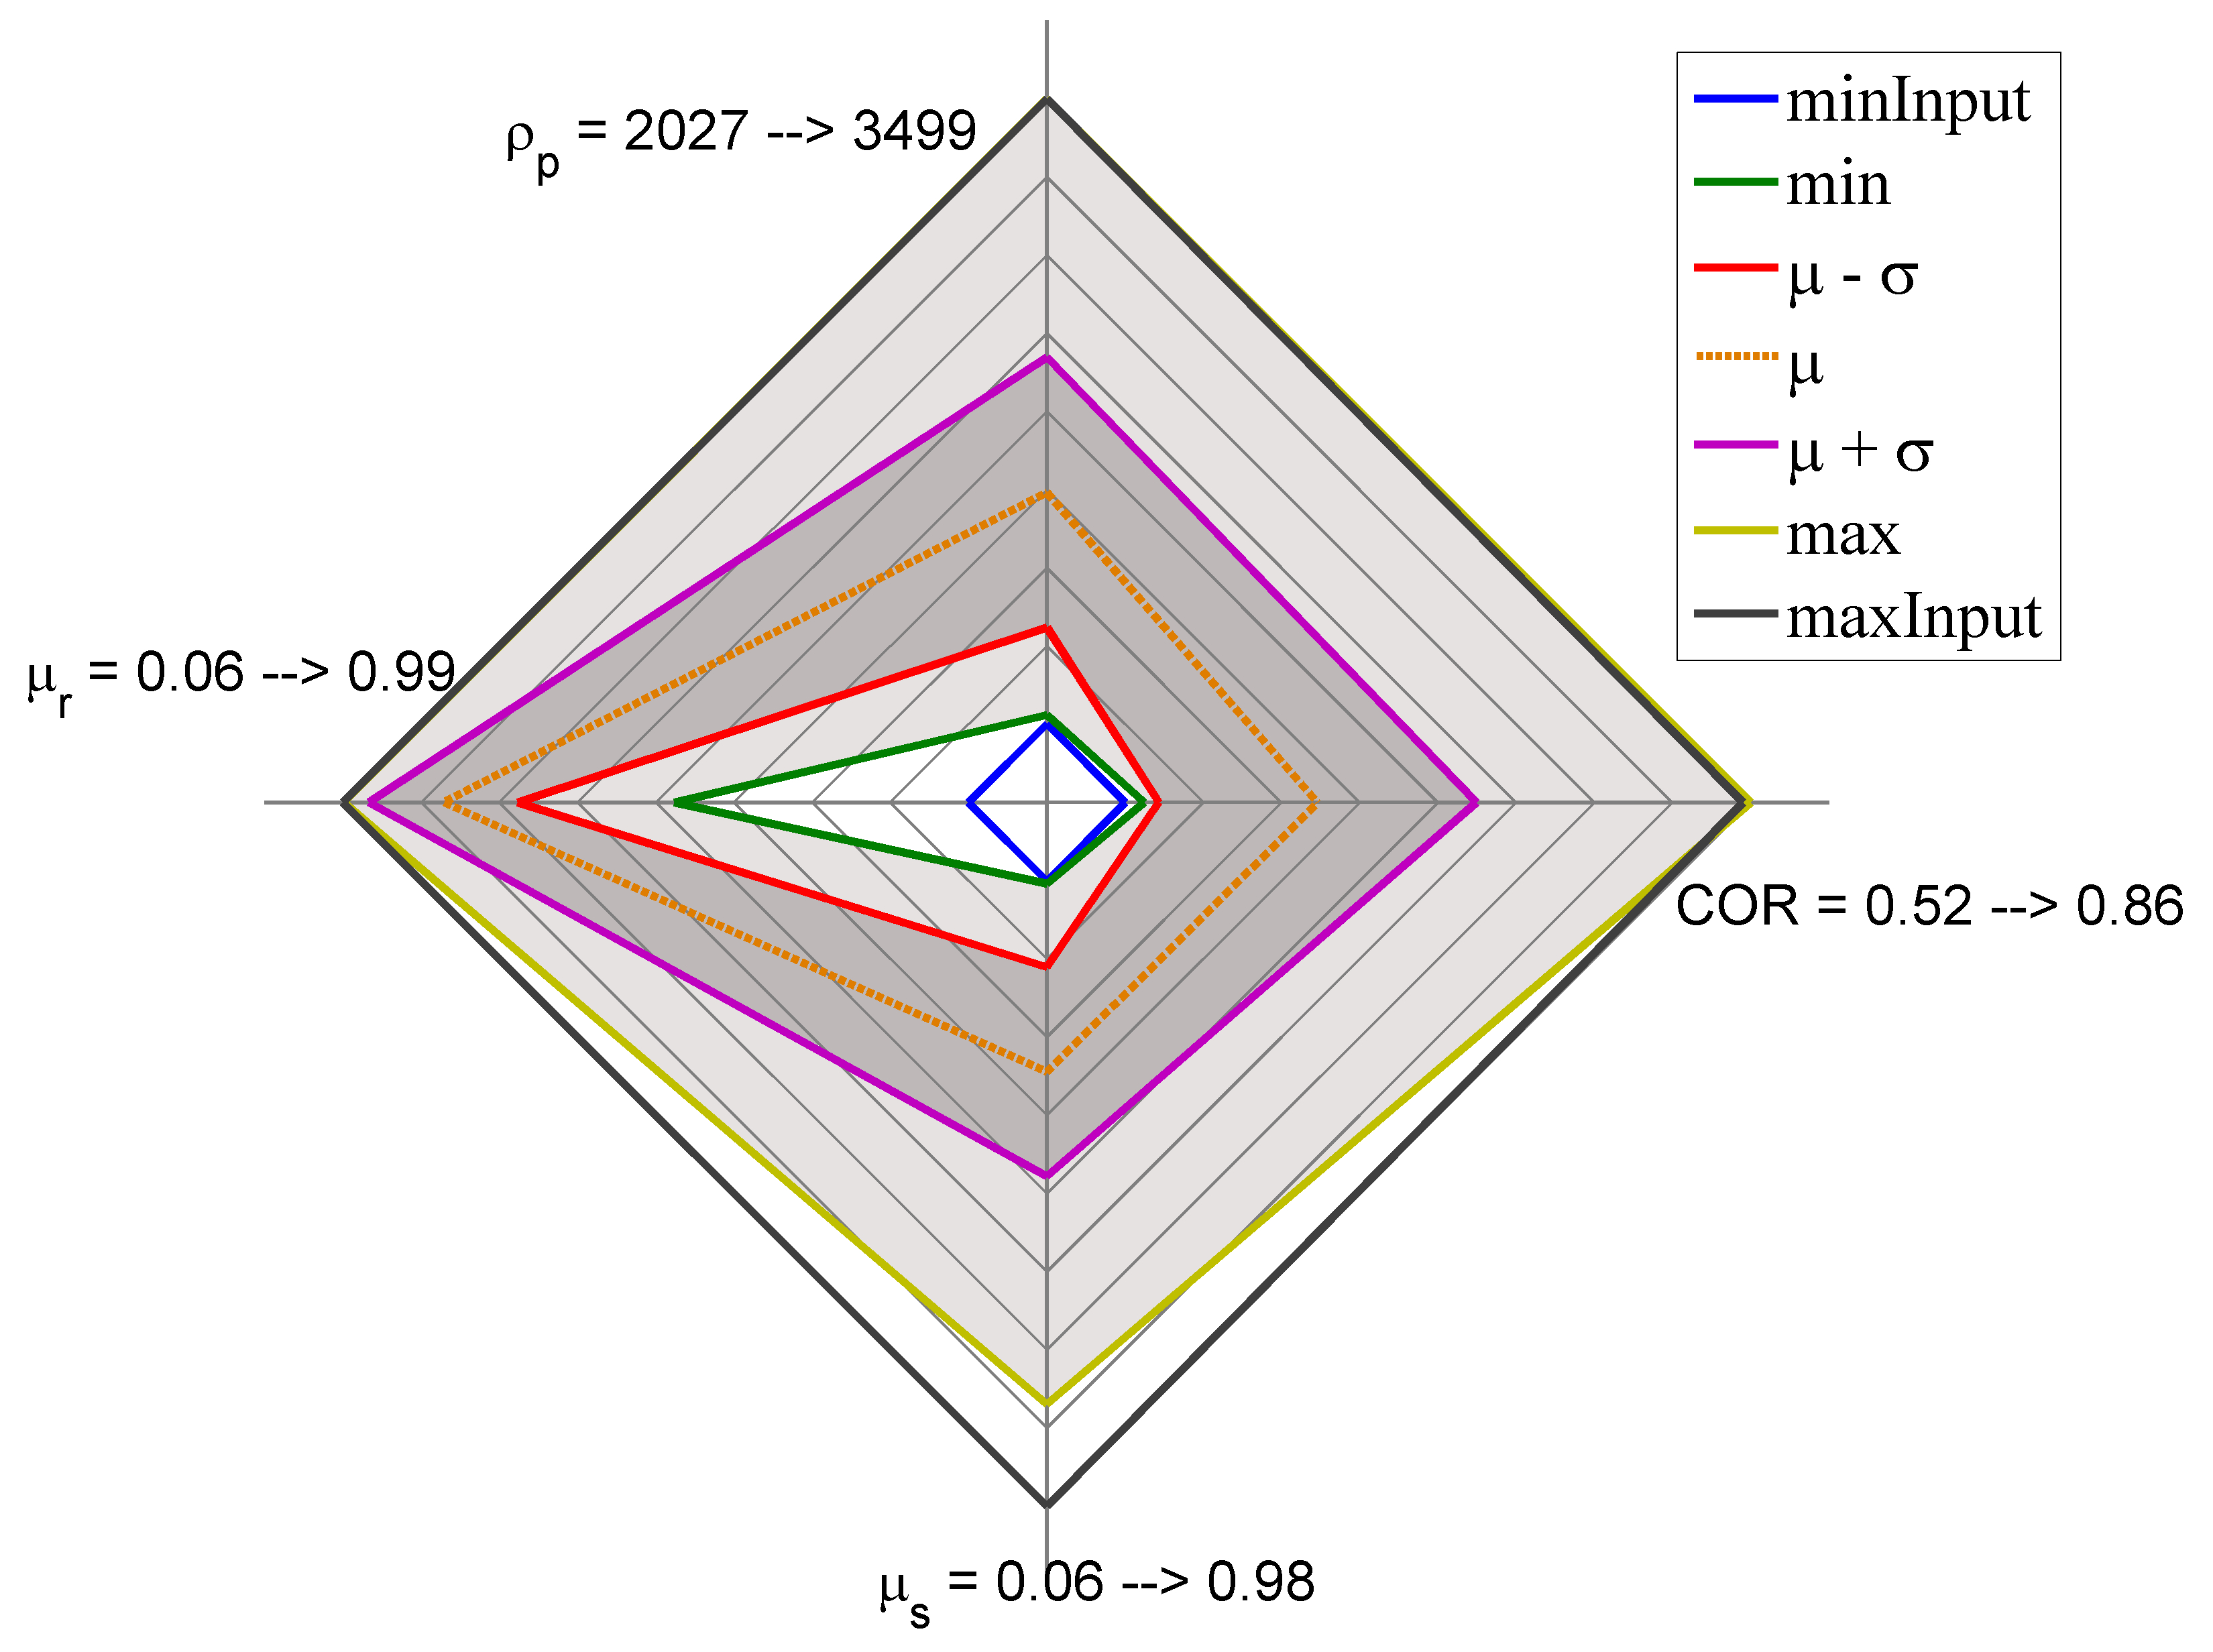
\includegraphics[width=\textwidth]{31radarpirker1aor}
        \caption{Parameter space plot, $AoR_{exp} = 38.85 ^\circ$}
        \label{fig:31radarpirker1aor} 
    \end{subfigure}\\
        \begin{subfigure}[b]{0.96\columnwidth}
        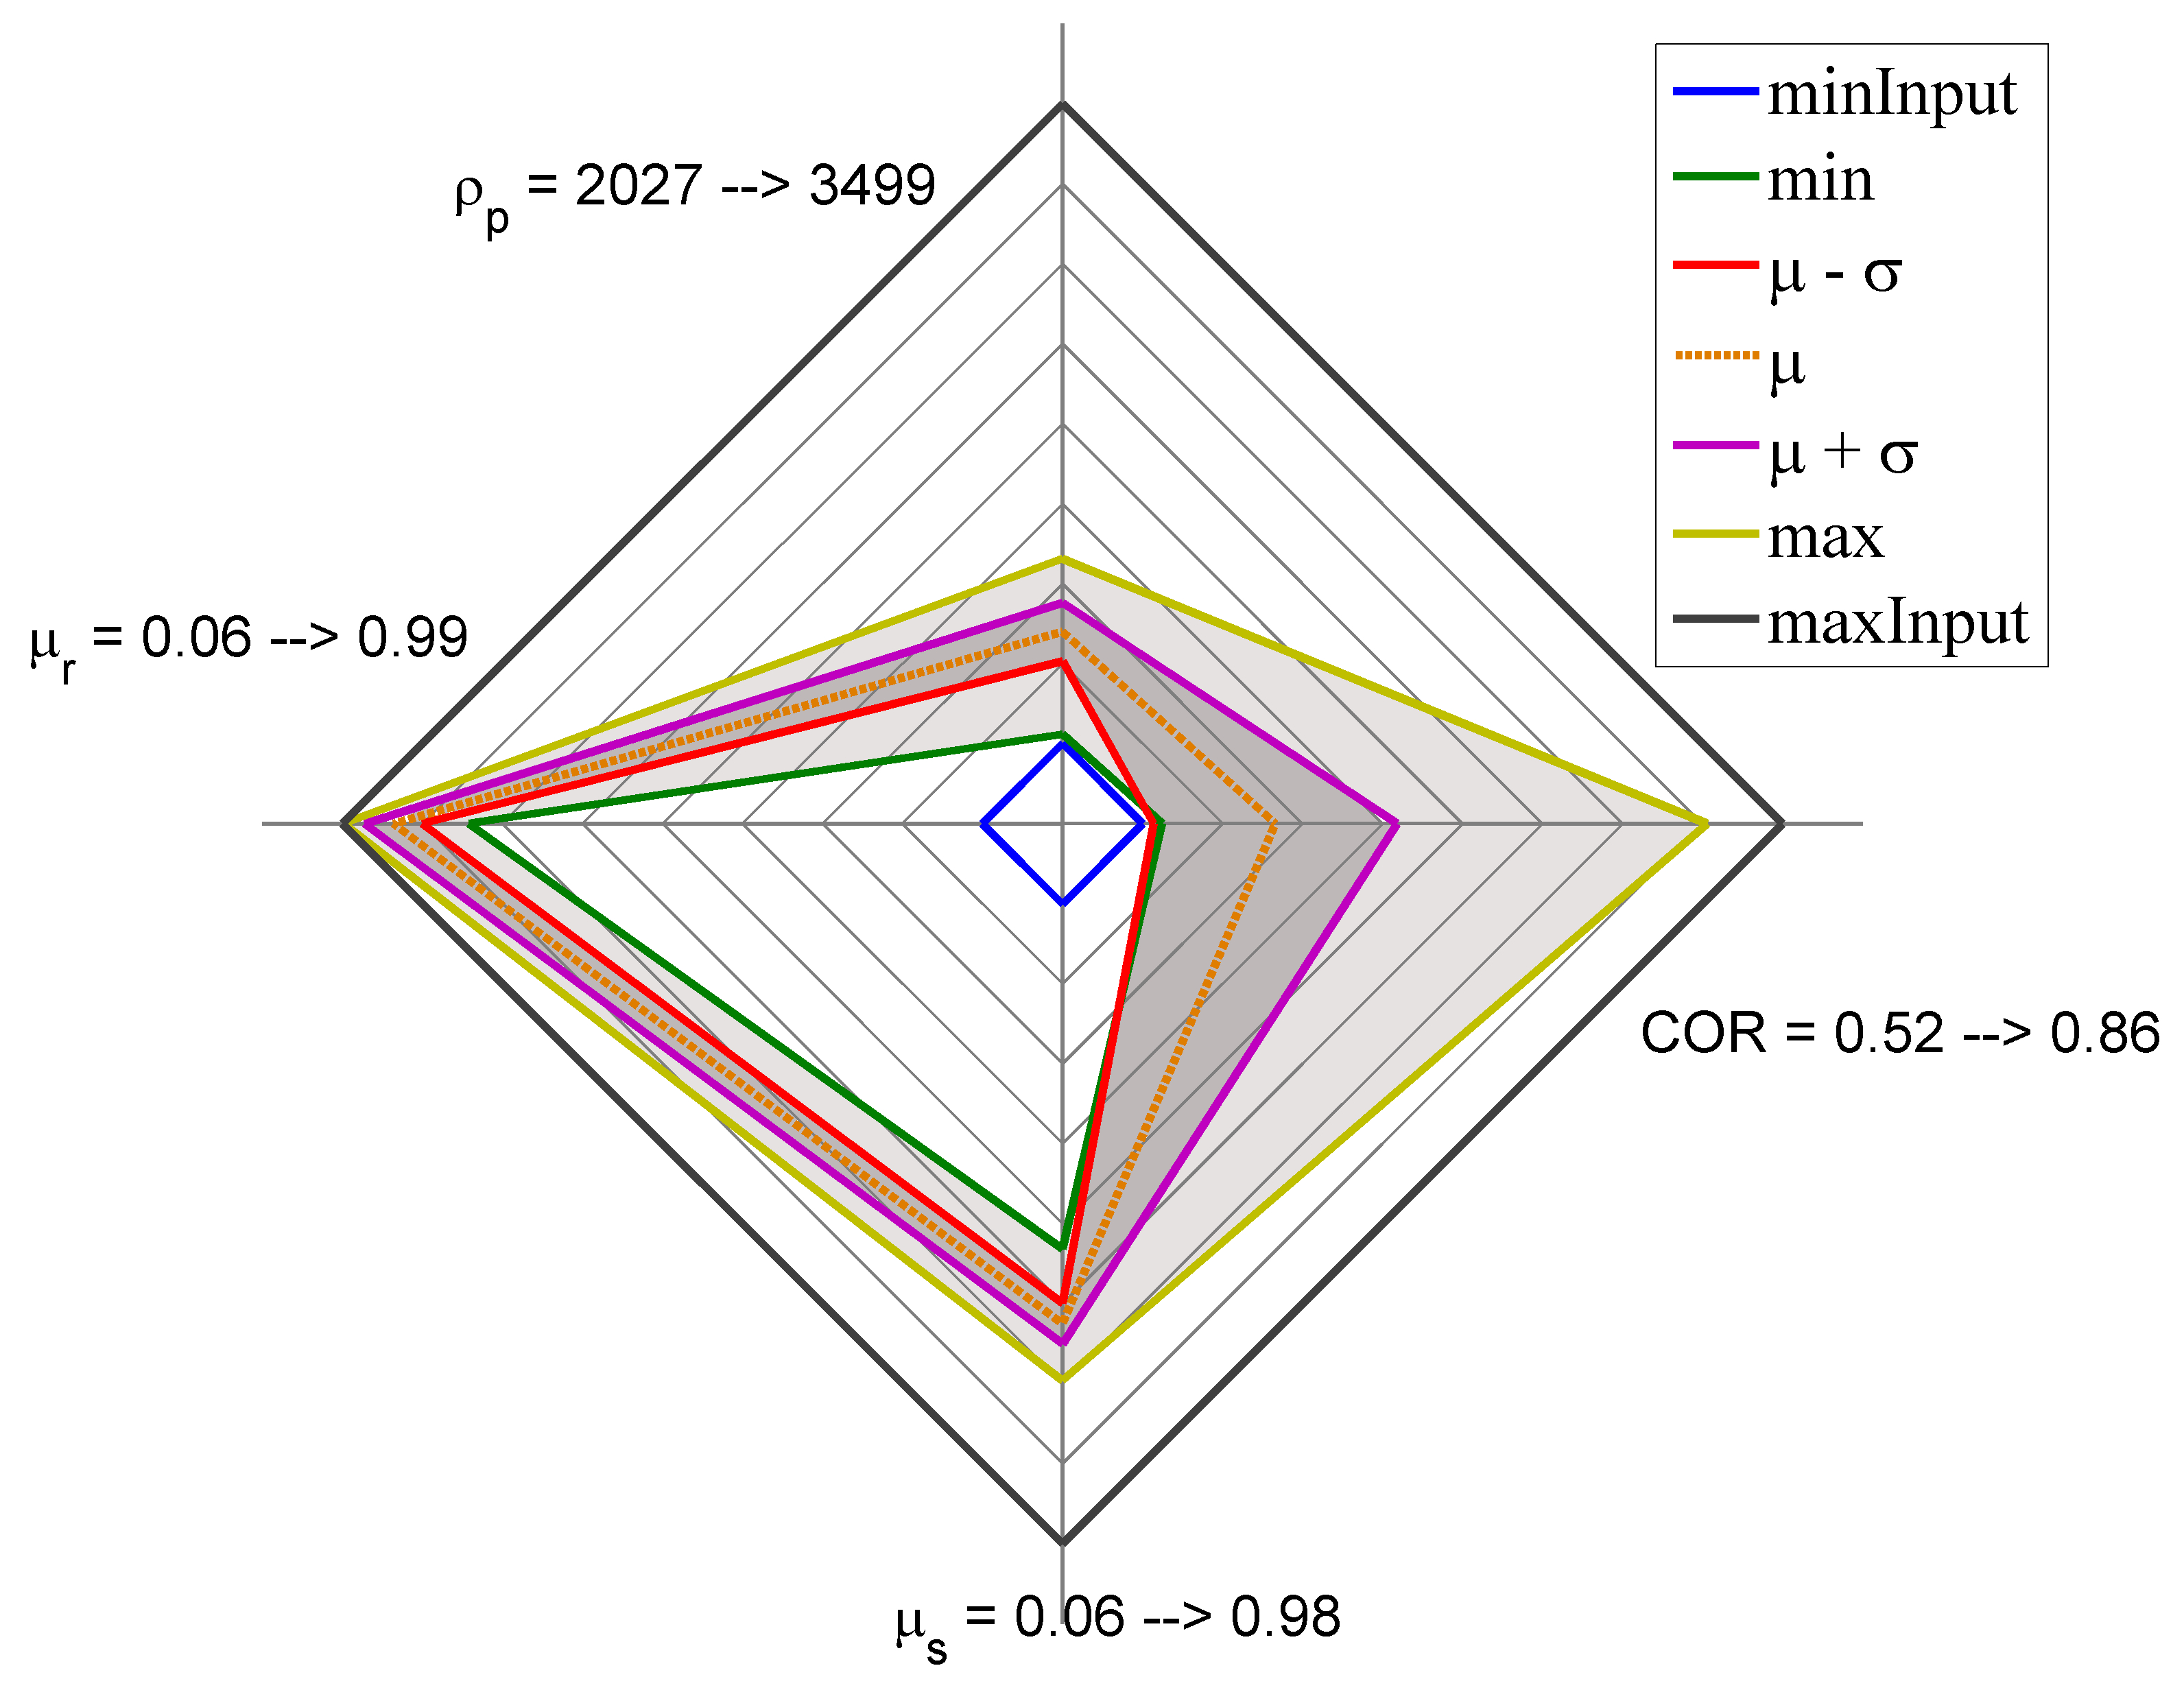
\includegraphics[width=\textwidth]{33radarpirker1schulze10070aor}
        \caption{Parameter space plot, $AoR_{exp} = 38.85
        ^\circ$ \& $SSC$: $\sigma_n=10070 ~[Pa]$}
        \label{fig:33radarpirker1schulze10070aor} 
    \end{subfigure}
    \caption[Parameter space plot of valid simulations parameters for the AOR and
    the merge between AOR and SCT valid parameters]{Parameter space plot of
    valid simulations parameters for the angle of repose tester ($AoR$) and the merge
    between AOR and shear cell tester ($SSC$).
    Each axis of the parameter space plot represents one simulation parameter.
    Furthermore, the shaded area represents valid parameters combinations.
    Dark shaded values stand for the confidence range.
    We represent the marked combinations for one load condition of the shear
    cell.
    Further explanation in the text. }
    \label{fig:35schulze10070aorradarandcloud}
\end{figure}